% !TEX root = thesis_draft.tex

\section{Inter-brain synchrony over time}
\label{sec:timecourse}

\begin{figure}[!htpb]
  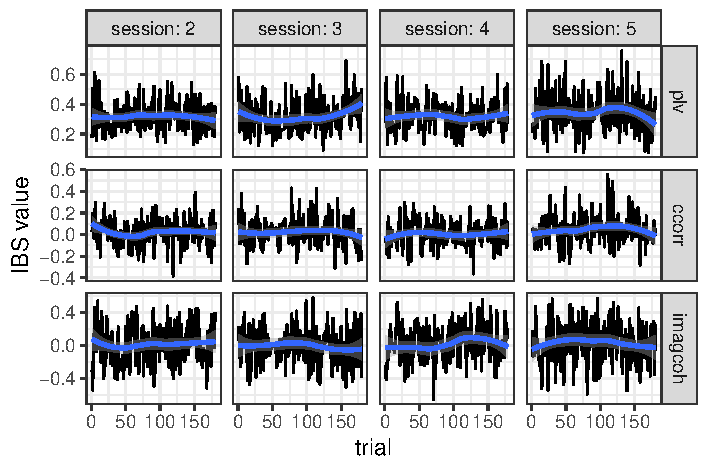
\includegraphics[width=\linewidth]{../stats/results/timecourse_repr.pdf}
  \caption{Development of inter-brain synchrony during the task. Variance is high, and there are no clear trends. (First 4 sessions only; alpha band; Pz electrode.)}
  \label{fig:timecourse_repr}
\end{figure}

\begin{figure}[!htpb]
  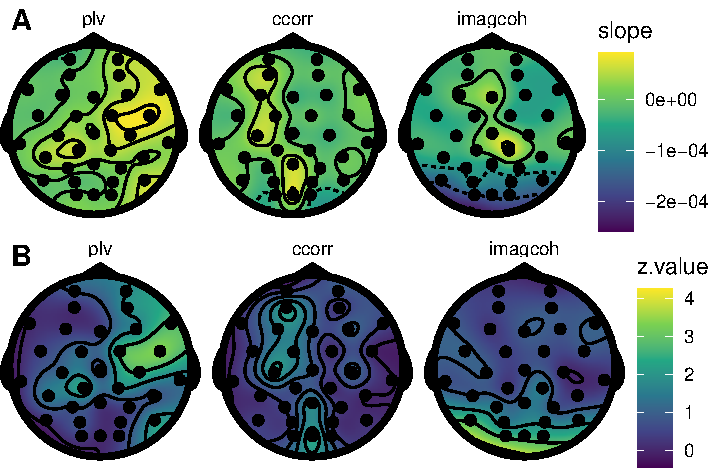
\includegraphics[width=\linewidth]{../stats/results/slopes_alpha.pdf}
  \caption{One inter-brain synchrony value is calculated per trial in the alpha band. (A) shows their (average) slope when we fit a line through them. (B) shows none of these slopes are significantly different from zero after FDR correction by comparing a linear mixed effect model that includes the slope to one that does not for each electrode.}
  \label{fig:slopes_alpha}
\end{figure}

\subsection{Introduction}

In \textcite{newman_effects_2021}'s experiment, participants need to converge on
a strategy to pick the same image or shape. As the task consists of two blocks, they
need to do so twice. We hypothesize more inter-brain synchrony (IBS) at the start of
a block, when participants need to figure out what the other is doing, and less
IBS towards the end, when participants will have switched to exploiting a by
then fixed strategy.

\subsection{Methods}

We first visualize IBS for a couple of representative sessions. Because we are
interested in effects over time that are potentially non-linear, we assess
their significance by comparing Generalized Additive Mixed Effect Models
\parencite[][GAMMs]{wood_generalized_2006} for each IBS measure. These models
contain two random effects: a factor smooth of trial by subject, and a factor
smooth of trial by electrode. This allows the model to generalize over session-
and electrode-specific trends in IBS values. GAMMs can deal with the structure
in the data caused by having multiple data points per dyad without requiring
averaging. To determine whether a given effect is significant, we add it as a
(smooth) fixed effect to one model, then compare both models.

Because it is potentially possible for effects to only show up in a couple
electrodes of interest, we additionally fit a (simpler) linear mixed effect
model with a random intercept per session on a subset of the data for each
combination of a measure and electrode. This allows us to see if there is a
linear effect of time within a session for each electrode and measure.

\subsection{Results}

Some representative timecourses of IBS data during the task are shown in
Figure~\ref{fig:timecourse_repr}. Just like with raw EEG data, there is high
variance and it can be hard to spot any trends without statistics or averaging.

No significant (smooth) effect of time (i.e. trial) was found for phase locking
value (PLV; $\chi^2(2) = 5.199, n.s.$), circular correlation
(CCorr;$\chi^2(2) = 5.862, n.s.$) or imaginary part of coherency (ImagCoh;
$\chi^2(2) = 3.734, n.s.$) in the alpha band. The same was true for the theta
band in the case of PLV ($\chi^2(2) = 4.982, n.s.$) and CCorr
($\chi^2(2) = 4.732, n.s.$), but not in the case of ImagCoh:
$\chi^2(2) = 5.805, p = 0.003$). This is due to an increase in ImagCoh values
towards the end of the second block. (A plot of the predicted values can be
found in the appendix, Figure~\ref{fig:imagcohtheta}.)

When looking at the electrode level in the alpha band, we see that the linear
effect of trial on IBS values is always close to zero
(Figure~\ref{fig:slopes_alpha}A). Unsurprisingly, none of these are
significant after FDR correction
(Figure~\ref{fig:slopes_alpha}B). It might appear as if that is not the case for
the bottom left of the ImagCoh plot, but this is an interpolation artifact:
z-values are only defined at the electrode positions. No effect of trial on IBS
was found at the electrode level in the theta band as well. (See
Figure~\ref{fig:slopes_theta} in the appendix).

\subsection{Discussion}

We found that contrary to our hypothesis, most IBS values in
\textcite{newman_effects_2021}'s experiment do not change over time, with the
possible exception of the ImagCoh values in the theta band. Interestingly, in
that case the effect was in a different direction than expected, with IBS
increasing towards the end of the block instead of going down.

One possible explanation is that performing the chosen strategy results in
similar brain activity in both participants, even if having theory of mind is
at that point no longer necessary. This could be due to performing the same
strategy, or simply due to shared environmental stimuli, like the end of the
experiment approaching. Alternatively, the assumption that towards
the end of a block participants will have converged on a strategy could be
incorrect. Finally, it is important to consider that the effect is not that big,
especially when taking into account only one out of six tests came out
significant. It could be a spurious result, especially as a robust result would
presumably be detectable by more than a single IBS measure. On the other hand,
ImagCoh is the only measure that includes amplitude information, so it could be
that it really found something the others are unable to.
\textcite{ayrolles_hypyp_2021} argue that amplitude information reflects
cognitive states better than phase information because of its larger timescale.
